\documentclass{standalone}
\usepackage{pgfplots}
\pgfplotsset{compat=1.13}
\usepackage{amsmath}

\begin{document}

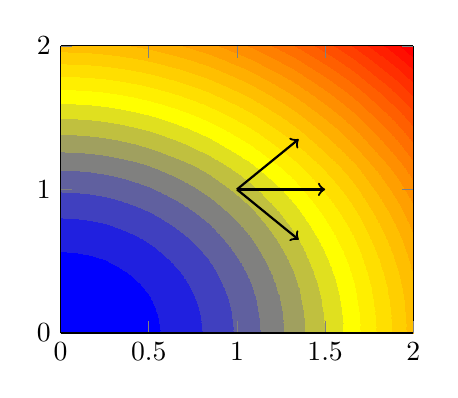
\begin{tikzpicture}
    \begin{axis}[
            view={0}{90},
            width = .5\textwidth]
        \addplot3[
            domain=0:2,
            domain y=0:2,
            contour filled={number=25}]
        {x*x + y*y};
        \draw[->,thick] (axis cs:1,1) -- (axis cs:1.35,1.35); %\node[midway, left]{\(\left(\begin{smallmatrix}0 \\ 1\end{smallmatrix} \right)\)};
        \draw[->,thick] (axis cs:1,1) -- (axis cs:1.5,1);
        \draw[->,thick] (axis cs:1,1) -- (axis cs:1.35,0.65);
    \end{axis}
\end{tikzpicture}

\end{document}